% Mathematical expression-tree regression derived from PGF grow' semantics.
\documentclass[border=2pt]{standalone}
\usepackage{tikz}
\usetikzlibrary{trees}

\tikzset{
  operator/.style={draw,circle,minimum size=8mm,inner sep=1pt,fill=purple!12},
  operand/.style={draw,rounded corners=2pt,minimum width=10mm,minimum height=7mm,inner sep=1pt},
  every edge from parent/.style={draw,thick}
}

\begin{document}
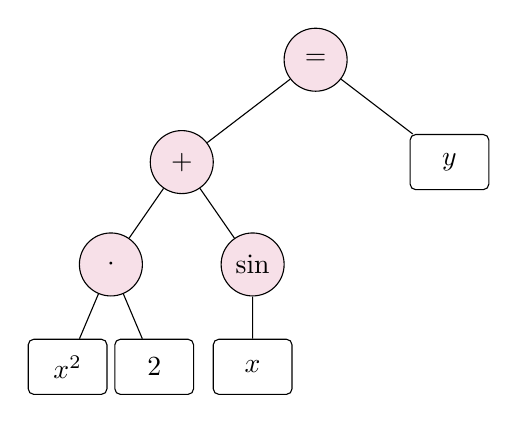
\begin{tikzpicture}[
  grow'=down,
  level distance=13mm,
  level 1/.style={sibling distance=34mm},
  level 2/.style={sibling distance=18mm},
  level 3/.style={sibling distance=11mm}
]
  \node[operator] {$=$}
    child {node[operand] {$y$}}
    child {
      node[operator] {$+$}
      child {
        node[operator] {$\sin$}
        child {node[operand] {$x$}}
      }
      child {
        node[operator] {$\cdot$}
        child {node[operand] {$2$}}
        child {node[operand] {$x^2$}}
      }
    };
\end{tikzpicture}
\end{document}
